\section{Positional encoding and training dynamics} \label{2506:sec:positional_encoding}
We now turn our attention to the role played by positional encoding in the attention layer when trained under SGD. Since the focus is on the effect of positional encoding, we stick with a class of target functions that can exhibit either a \emph{semantic} (label mostly depends on tokens value, but not the order) or a \emph{positional} (where tokens most important feature is their position in the sequence, rather than their embedding). Consider an SSI target function of the form
\begin{equation} \label{2506:eq:positional-semantic-label}
    \vec{f}^\mathrm{SSI}_{\vec w_{\star}}(X) = (1-\omega) \SoftMax\left(X\vec{w}_\star \vec{w}_\star^\top X^\top\right) + \omega \SoftMax\left[\begin{pmatrix}
        a^2 & -a^2 \\
        -a^2 & a^2 \\
    \end{pmatrix}\right]
    \in \mathbb{R}^{2\times 2},
\end{equation}
where the parameter $\omega\in[0,1]$ allows the target to switch from a semantic to a positional behavior, while the parameter $a\in(0,1]$ controls the alignment of the target with its positional part.

We shall train the model in Equation~\eqref{2506:eq:model-definition} with positional encoding
\(P_1 = -P_2\)
and reduction map \(R\) the identity function. We focus on the \emph{gradient flow} limit where $\eta$ is sufficiently small \citep{chung1954stochastic}. Our analysis will focus on the population loss given by Equation~\eqref{2506:eq:population-loss_sufficient-statistic}, since it completely characterize the behavior of SGD in this regime; the sufficient statistics \((\vec{e},m)\) are the only free variables of the setting.

The sequential information exponent of this setting is \(\mathrm{SIE}=2\) (see Appendix~\ref{2506:app:further-positional-demantic} for the explicit derivation), thus the sample complexity for escaping the initialization is \(\mathcal{O}(d \log d)\).
After the initial phase, SGD fast converges to the minimum of the population loss that is fully aligned with either the semantic or the positional sufficient statistic, i.e. \(\norm{(\vec{e},m)} = 1\), but is not guaranteed to be the global minimum. 
Figure~\ref{2506:fig:positional-semantic-trajectories-a1} shows an example where the population loss has 2 minimums, one semantic with \((e,m)=(1,0)\) and one positional with \((e,m)=(0,1)\), and the steepest direction at initialization, namely the eigenvector associated with the lowest eigenvalue of the Hessian, points towards the local one; in this case, the gradient flow will converge to the wrong minima.

Varying the parameters, \(\omega\) and \(a\) the high-dimensional SGD dynamics from random initialization exhibits a rich phenomenology. In Figure~\ref{2506:fig:phase-diagram-postional-semantic} we show the phase diagram with all the possible behaviors:
\begin{itemize}
    \item \textbf{\color{UniquePositionalMinima} Unique Positional Minima}: the population loss has unique positional minima, and the SGD converges to it. This is the case for \(\omega=1\) and \(a=1\).
    \item \textbf{\color{GlobalPositionalMinima} Global Positional Minima}: the population loss has both a semantic and a positional minimum, and SGD converges to the global positional one.
    \item \textbf{\color{GlobalSemanticMinimaPositionalDynamic} Global Semantic Minima, Positional Dynamic}: the population loss has both a semantic and a positional minimum, and SGD converges to the local positional one. This is the case where SGD \textbf{does not converge} to the global minima.
    \item \textbf{\color{UniqueSemanticMinimaMisalignedDynamic} Unique Semantic Minima, Misaligned Dynamics}: the population loss has unique semantic minima, and the SGD converges to it, even though the steepest direction at initialization points orthogonal to it.
    \item \textbf{\color{GlobalSemanticMinima} Global Semantic Minima}: the population loss has both a semantic and positional minima, and SGD converges to the global semantic one.
    \item \textbf{\color{UniqueSemanticMinima} Unique Semantic Minima}: the population loss has unique semantic minima, and the SGD converges to it. This is the case for \(\omega=0\) and \(a=1\).
\end{itemize}

\begin{figure}
    \centering
    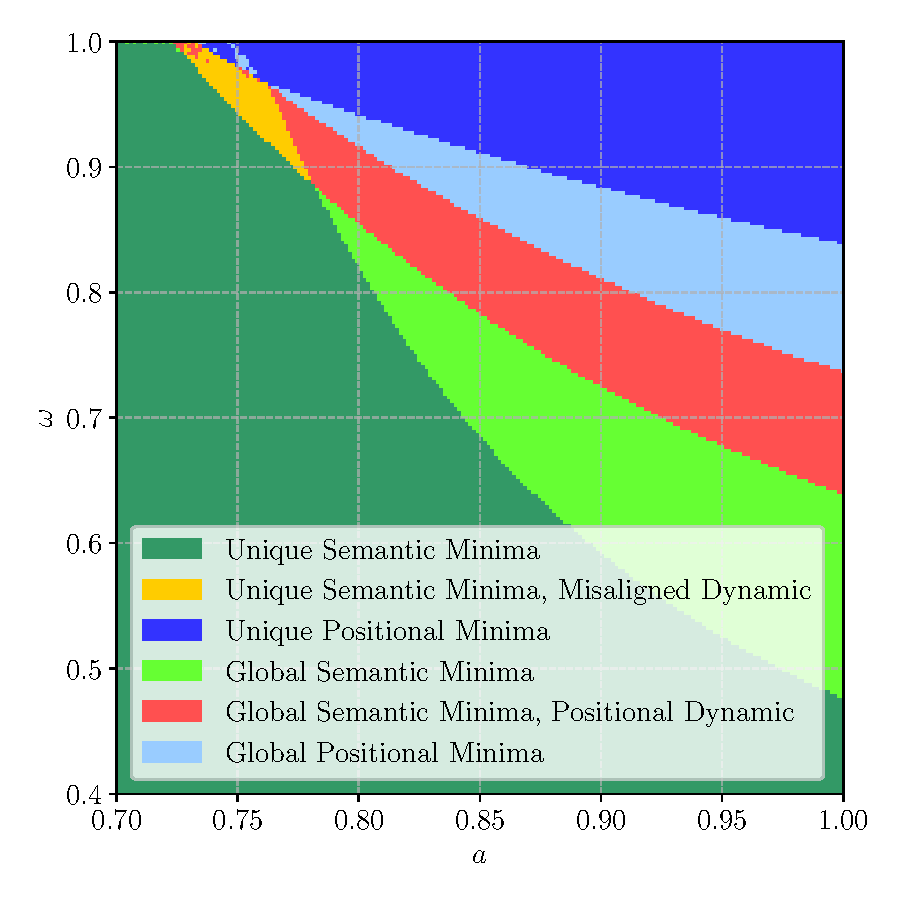
\includegraphics[width=0.49\textwidth]{figs/positional-semantic/phase_diagram}
    \caption{Different behaviors of SGD depending on the parameters \(\omega\) and \(a\).}
    \label{2506:fig:phase-diagram-postional-semantic}
\end{figure}
We verify this by simulating many runs of SGD with different initializations and data samples. In Figure~\ref{2506:fig:positional-semantic-trajectories-a1} we compute the empirical probability of convergence to the semantic minima, for \(a=1\) and varying \(\omega\).
The theoretical value of \(\omega\) where we have a transition from  sematic to positional dynamics is \(\omega_\mathrm{trans} = 0.64\), which is in good agreement with the transition observed in the measured probabilities; the transition becomes sharper as \(d\) increases: ideally, in the limit \(d\to\infty\) we expect a step function. The simulations in Figure~\ref{2506:fig:positional-semantic-trajectories-a1} are performed with \(d=1000\), and some finite size effects are still present. In Appendix~\ref{2506:app:further-positional-demantic} we show present a more detailed analysis, including different values of \(d\).

\begin{figure}
    \centering
    % 
    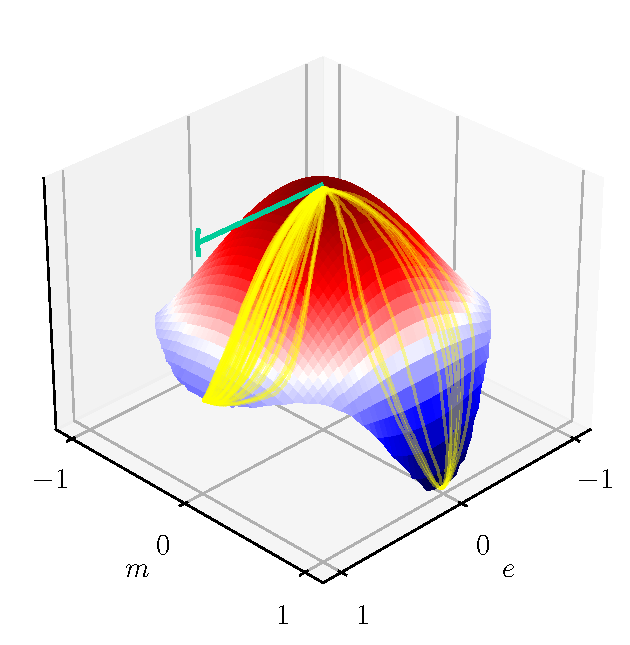
\includegraphics[height=0.49\textwidth]{figs/positional-semantic/loss_surface_omega0.67_a1}
    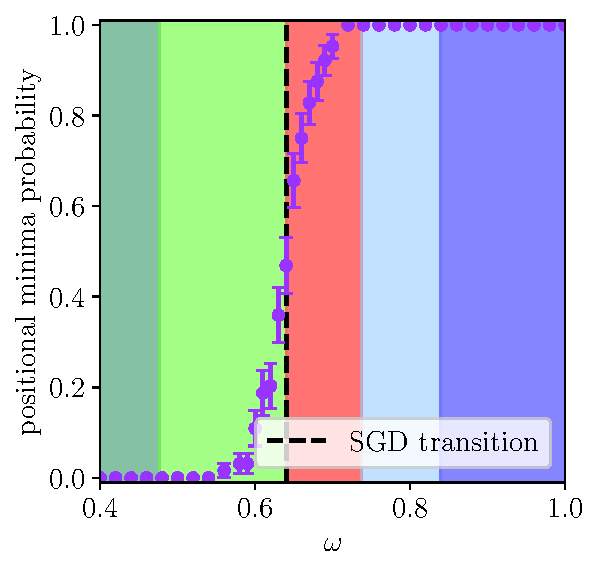
\includegraphics[height=0.49\textwidth]{figs/positional-semantic/trajectories-probability}
    \caption{
        (left) surface of the population loss for \(\omega = 0.67\) and \(a=1\). The steepest direction at initialization (green vector) points towards the \emph{positional} local minimum, while the global minima is semantic.
        Some examples of SGD trajectories are shown in yellow: most of them fall into the semantic local minimum, while some others manage to fully-recover the global minimum due to finite size effects (\(d=1000\)).
        %
        (right) empirical probability of convergence to the semantic minima as a function of \(\omega\) for \(a=1\). The probability is computed over 64 SGD runs with different initializations and data samples. The theoretical prediction of the transition from semantic to positional minima is at \(\omega_\mathrm{trans}\approx0.64\). 
    }
    \label{2506:fig:positional-semantic-trajectories-a1}
\end{figure}
